\chapter{Pattern Matching}

\section{Hubungan antara Elixir, Erlang, dan BEAM}

Diagram berikut menggambarkan hubungan antara Elixir, Erlang, dan BEAM:

\begin{center}
	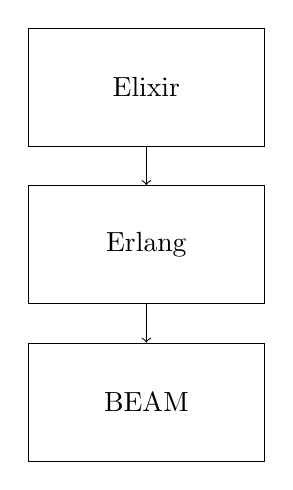
\begin{tikzpicture}[node distance=2cm]
		\node (elixir) [rectangle, draw, text centered, minimum height=1.5cm, minimum width=3cm] {Elixir};
		\node (erlang) [rectangle, draw, below of=elixir, text centered, minimum height=1.5cm, minimum width=3cm] {Erlang};
		\node (beam) [rectangle, draw, below of=erlang, text centered, minimum height=1.5cm, minimum width=3cm] {BEAM};
		
		\draw[->] (elixir) -- (erlang);
		\draw[->] (erlang) -- (beam);
	\end{tikzpicture}
\end{center}

\subsection{Elixir}

Elixir adalah bahasa pemrograman yang modern dan dinamis, dikembangkan untuk memenuhi kebutuhan aplikasi terdistribusi yang skalabel dan fault-tolerant. Meskipun Elixir memiliki sintaks yang berbeda dan modern, ia bergantung sepenuhnya pada ekosistem Erlang untuk menjalankan aplikasinya.

\subsection{Erlang}

Erlang adalah bahasa pemrograman yang mendasari Elixir. Ketika kode Elixir dikompilasi, ia diubah menjadi bytecode Erlang. Ini memungkinkan Elixir untuk memanfaatkan seluruh ekosistem Erlang, termasuk pustaka, alat, dan framework yang sudah ada. Dengan kata lain, Elixir adalah lapisan di atas Erlang yang menyediakan sintaks dan fitur tambahan sambil tetap menggunakan fondasi yang kuat dari Erlang.

\subsection{BEAM}

BEAM (Bogdan/Björn's Erlang Abstract Machine) adalah mesin virtual yang menjalankan bytecode Erlang, termasuk kode yang ditulis dalam Elixir. BEAM dirancang untuk mendukung concurrency, fault-tolerance, dan distribusi yang dibutuhkan oleh aplikasi Elixir dan Erlang. BEAM adalah komponen inti yang membuat Elixir dan Erlang mampu menangani jutaan proses secara efisien.

\subsection{Hubungan dalam Diagram}

Diagram di atas menunjukkan bagaimana Elixir bergantung pada Erlang dan akhirnya dijalankan di atas BEAM. Ketika seorang pengembang menulis kode dalam Elixir, kode tersebut pertama-tama diterjemahkan menjadi bytecode Erlang. Selanjutnya, bytecode tersebut dijalankan oleh BEAM, yang mengelola eksekusi program secara efisien. Ini berarti meskipun Elixir dan Erlang adalah bahasa yang berbeda, mereka berbagi mesin runtime yang sama, yaitu BEAM, yang membuat mereka sangat kompatibel dan interoperabel.

\section{Pattern Matching di Elixir}

Pattern matching adalah salah satu fitur paling kuat dan fundamental dalam bahasa pemrograman Elixir. Fitur ini memungkinkan pengembang untuk mencocokkan struktur data dan mengekstrak nilai-nilai dari struktur tersebut secara deklaratif. Tidak seperti bahasa pemrograman imperatif di mana variabel diinisialisasi dengan nilai, dalam Elixir, pattern matching berfungsi sebagai alat untuk membandingkan dan mengurai data.

\subsection{Dasar-Dasar Pattern Matching}

Pada dasarnya, pattern matching menggunakan operator \texttt{=} untuk mencocokkan sisi kiri dan sisi kanan dari ekspresi. Jika keduanya cocok, maka Elixir akan mengikat nilai dari sisi kanan ke variabel di sisi kiri.

\begin{lstlisting}[language=Elixir]
	iex> x = 1
	1
	
	iex> 1 = x
	1
\end{lstlisting}

Dalam contoh di atas, nilai 1 di sisi kanan diikat ke variabel \texttt{x}. Karena sisi kiri dan kanan dari ekspresi \texttt{1 = x} cocok, Elixir hanya mengembalikan \texttt{1}.

\subsection{Pattern Matching dengan Tuple}

Pattern matching sangat berguna ketika bekerja dengan struktur data yang lebih kompleks seperti tuple.

\begin{lstlisting}[language=Elixir]
	iex> {a, b, c} = {1, 2, 3}
	{1, 2, 3}
	
	iex> a
	1
	
	iex> b
	2
	
	iex> c
	3
\end{lstlisting}

Dalam contoh di atas, tuple \texttt{\{1, 2, 3\}} dicocokkan dengan pola \texttt{\{a, b, c\}}, sehingga nilai-nilai di dalam tuple diikat ke variabel \texttt{a}, \texttt{b}, dan \texttt{c}.

\subsection{Pattern Matching dengan List}

Pattern matching juga dapat digunakan dengan list, termasuk penggunaan \texttt{head} dan \texttt{tail} untuk mencocokkan bagian pertama dari list dan sisa elemennya.

\begin{lstlisting}[language=Elixir]
	iex> [head | tail] = [1, 2, 3]
	[1, 2, 3]
	
	iex> head
	1
	
	iex> tail
	[2, 3]
\end{lstlisting}

Di sini, \texttt{head} mendapatkan nilai pertama dari list, sedangkan \texttt{tail} mendapatkan list yang tersisa.

\subsection{Menggunakan Pattern Matching dalam Fungsi}

Pattern matching dapat digunakan dalam definisi fungsi untuk membuat kode yang lebih bersih dan mudah dibaca.

\begin{lstlisting}[language=Elixir]
	defmodule Example do
	def greet({first_name, last_name}) do
	"Hello, #{first_name} #{last_name}!"
	end
	end
	
	iex> Example.greet({"John", "Doe"})
	"Hello, John Doe!"
\end{lstlisting}

Pada contoh ini, fungsi \texttt{greet/1} menerima tuple yang terdiri dari \texttt{first\_name} dan \texttt{last\_name}. Nilai-nilai ini langsung dicocokkan dengan pola yang didefinisikan dalam parameter fungsi.

Pattern matching di Elixir memungkinkan pemrograman yang lebih deklaratif dan ekspresif. Dengan kemampuan untuk mencocokkan dan mengurai struktur data, pattern matching menjadi salah satu fitur esensial yang mempermudah pengembangan aplikasi dalam Elixir.



\section{Pattern Pipe Operator di Elixir}

\textit{Pipe operator} (\texttt{|>}) adalah salah satu fitur yang sangat berguna di Elixir, yang memungkinkan chaining atau penggabungan dari beberapa operasi menjadi satu alur yang mudah dibaca. Pipe operator mengambil output dari ekspresi sebelumnya dan meneruskannya sebagai argumen pertama ke fungsi berikutnya.

\subsection{Dasar-Dasar Pipe Operator}

Pada dasarnya, pipe operator memungkinkan kita untuk menulis kode yang lebih rapi dan berurutan daripada harus menyusun fungsi secara bersarang (nested).

\begin{lstlisting}[language=Elixir]
	iex> "hello"
	...> |> String.upcase()
	...> |> String.reverse()
	"OLLEH"
\end{lstlisting}

Dalam contoh di atas, string \texttt{"hello"} pertama-tama diubah menjadi huruf kapital dengan \texttt{String.upcase/1}, kemudian hasilnya diteruskan ke \texttt{String.reverse/1} yang membalikkan urutan karakter. Tanpa pipe operator, kode ini akan terlihat seperti berikut:

\begin{lstlisting}[language=Elixir]
	iex> String.reverse(String.upcase("hello"))
	"OLLEH"
\end{lstlisting}

\subsection{Pipe Operator dengan List}

Pipe operator juga sering digunakan dengan fungsi-fungsi yang memanipulasi list, seperti pada contoh berikut:

\begin{lstlisting}[language=Elixir]
	iex> [1, 2, 3, 4, 5]
	...> |> Enum.map(&(&1 * 2))
	...> |> Enum.filter(&(&1 > 5))
	[6, 8, 10]
\end{lstlisting}

Pada contoh ini, list \texttt{[1, 2, 3, 4, 5]} pertama-tama dikalikan dengan 2 menggunakan \texttt{Enum.map/2}, kemudian hasilnya disaring dengan \texttt{Enum.filter/2} untuk hanya menyertakan angka yang lebih besar dari 5.

\subsection{Penjelasan `\&1`, `\&2`, dan Seterusnya}

Dalam Elixir, `\&` digunakan untuk membuat anonymous functions atau fungsi tanpa nama. Dalam anonymous function, `\&1`, `\&2`, dan seterusnya adalah placeholder untuk argumen yang diterima oleh fungsi tersebut.

\begin{lstlisting}[language=Elixir]
	iex> add = &(&1 + &2)
	#Function<6.86581258/2 in :erl_eval.expr/5>
	iex> add.(2, 3)
	5
\end{lstlisting}

Pada contoh ini, `\&1` dan `\&2` mewakili argumen pertama dan kedua dari anonymous function yang dibuat. Fungsi ini menambahkan kedua argumen dan mengembalikan hasilnya.

Pipe operator di Elixir mempermudah penulisan kode yang jelas dan mudah dibaca, terutama ketika menggabungkan serangkaian operasi. Selain itu, kemampuan untuk menggunakan pipe operator dengan fungsi yang menerima banyak parameter serta penggunaan `\&1`, `\&2`, dan seterusnya memungkinkan penulisan kode yang lebih fleksibel dan ekspresif.

\subsection{Pipe Operator dengan Fungsi yang Memiliki Banyak Parameter}

Pipe operator juga dapat digunakan dengan fungsi yang memerlukan lebih dari satu parameter. Berikut adalah contohnya:

\begin{lstlisting}[language=Elixir]
	defmodule Example do
	def multiply_and_add(x, y, z) do
	x * y + z
	end
	end
	
	iex> 5
	...> |> Example.multiply_and_add(2, 3)
	13
\end{lstlisting}

Dalam contoh di atas, angka \texttt{5} diteruskan sebagai parameter pertama ke fungsi \texttt{multiply\_and\_add/3}, dan parameter kedua dan ketiga adalah \texttt{2} dan \texttt{3}. Fungsi ini mengalikan \texttt{5} dengan \texttt{2} dan menambahkan \texttt{3}, menghasilkan \texttt{13}.



\subsection{Contoh dengan Konversi Tipe Data}

Dalam Elixir, ketika kita menggunakan pipe operator dengan fungsi yang memerlukan parameter dengan tipe yang berbeda dari output fungsi sebelumnya, kita harus memastikan bahwa data yang diteruskan sesuai dengan tipe yang diharapkan oleh fungsi tersebut. Ini mungkin memerlukan konversi atau pemrosesan data sebelum menggunakan pipe operator.

Misalkan kita memiliki fungsi yang mengharapkan parameter bertipe integer dan fungsi lain yang menghasilkan string. Kita perlu mengkonversi string menjadi integer sebelum meneruskan ke fungsi berikutnya.

Berikut adalah contoh sederhana:

\begin{lstlisting}[language=Elixir]
	defmodule Converter do
	def string_to_integer(str) do
	String.to_integer(str)
	end
	
	def add_five(num) do
	num + 5
	end
	end
	
	iex> "42"
	...> |> Converter.string_to_integer()
	...> |> Converter.add_five()
	47
\end{lstlisting}

Pada contoh ini, string \texttt{"42"} pertama-tama dikonversi menjadi integer dengan \texttt{Converter.string\_to\_integer/1}, kemudian hasil integer tersebut diteruskan ke \texttt{Converter.add\_five/1} untuk ditambahkan dengan 5.

\subsection{Menggunakan Nilai Pipe sebagai Parameter Kedua}

Di Elixir, kita dapat menggunakan pipe operator untuk meneruskan nilai dari fungsi pertama sebagai parameter kedua dalam sebuah fungsi dengan memanfaatkan fungsi anonim. Contoh berikut menunjukkan cara melakukannya:

\begin{lstlisting}[language=Elixir]
	defmodule Example do
	def hello(greet, name) do
	greet <> name
	end
	end
	
	iex> "world"
	...> |> (&Example.hello("Hello, ", &1 )).()
	"Hello, world"
\end{lstlisting}

Pada kode di atas, modul \texttt{Example} mendefinisikan fungsi \texttt{hello/2} yang menggabungkan dua string: \texttt{greet} dan \texttt{name}. Nilai \texttt{"world"} diteruskan melalui pipe operator ke fungsi anonim. Fungsi anonim tersebut menggunakan \texttt{"Hello, "} sebagai parameter pertama dan nilai dari pipe (\texttt{"world"}) sebagai parameter kedua. 

Fungsi \texttt{hello/2} kemudian menggabungkan \texttt{"Hello, "} dengan \texttt{"world"}, menghasilkan string \texttt{"Hello, world"}. Dengan pendekatan ini, pipe operator dan fungsi anonim memungkinkan kita untuk dengan mudah mengatur parameter fungsi, termasuk menggunakan nilai dari pipe sebagai parameter kedua. Pendekatan ini meningkatkan fleksibilitas dan keterbacaan kode dalam Elixir.

